{\bfseries IRSTI 28.23.37}

\sectionwithauthors{Т.Р Жабаев, У.А.Тукеев}{STUDY OF THE REPRESENTATIVENESS OF KAZAKH LANGUAGE CORPORA BY
WORD STEMS FOR THE SUMMARIZATION TASK}

\begin{center}
{\bfseries Т.Р Жабаев, У.А.Тукеев}

Kazakh National University named after al-Farabi, Almaty, Kazakhstan,

е-mail:talgat14430@gmail.com
\end{center}

The aim of the work is to prove the possibility of determining the
representativeness of a corpus for training a neural model before
conducting resource-intensive experiments. In this work, we investigated
the dependence of the summarization model on the number of word stems in
it. The work was carried out on a synthetic summarization dataset for
the Kazakh language. Taking the number of word stems as the
representativeness metric, an analysis of the quality of the work of
three summarization models was performed depending on the number of word
stems in the training dataset. These training datasets differ in the
number of rows. To obtain these datasets, we split the training dataset
into three parts of different sizes. On the test files, BLEU scores were
obtained for each model during the inference process. The highest BLEU
scores are obtained for the model trained on the largest amount of data.
When the train dataset was reduced by 50 percent, the score decreased
from 4 to 25. On the smallest dataset, the score dropped from 25 to 31.
The experimental part of the work showed that the model with the largest
number of stems shows the highest BLEU score. The scientific
contribution of the work is the experimental proof of the
representativeness of the training corpus by the number of stems before
training the neural model.

{\bfseries Keywords}: neural language modeling, NLP, text summarization,
Kazakh language, representativity, synthetic datasets.

\begin{center}
{\large\bfseries ЖИНАҚТАУ ТАПСЫРМАСЫ БОЙЫНША ҚАЗАҚ ТІЛІ КОРПУСЫНЫҢ СӨЗ}

{\bfseries ТҮБІРЛЕРІ БОЙЫНША РЕПРЕЗЕНТАТИВТІЛІГІН ЗЕРТТЕУ}

{\bfseries Т.Р.Жабаев, У.А.Тукеев}

әл-Фараби атындағы Қазақ ұлттық университеті, Алматы, Казахстан,

е-mail:talgat14430@gmail.com
\end{center}

Жұмыстың мақсаты -- ресурсты көп қажет ететін эксперименттер жүргізу
алдында нейрондық модельді оқыту үшін корпустың репрезентативтілігін
анықтау мүмкіндігін дәлелдеу. Бұл жұмыста біз жинақтау моделінің
жұмысының сөз түбірлерінің санына тәуелділігін зерттедік. Жұмыс қазақ
тіліне арналған синтетикалық жинақтау деректер жинағы бойынша орындалды.
Сөз түбірлерінің санын репрезентативтілік көрсеткіші ретінде ала отырып,
оқу деректер жинағындағы сөз түбірлерінің санына байланысты үш жинақтау
моделінің жұмыс сапасына талдау жасалды. Бұл оқу деректер жинағы жолдар
саны бойынша ерекшеленеді. Бұл деректер жиынын алу үшін біз оқыту
деректер жинағын әртүрлі өлшемдегі үш бөлікке бөлеміз. Әр модель үшін
BLEU бағалаулары қорытынды жасау барысында сынақ файлдарын пайдалана
отырып алынды. Деректердің ең үлкен көлемі бойынша дайындалған модельде
ең жоғары BLEU ұпайлары болды. Окыті деректер жинағы 50 пайызға азайған
кезде балл 4-тен 25-ке дейін төмендеді. Ең кішкентай деректер жиынында
балл 25-тен 31-ге дейін төмендеді. Жұмыстың эксперименттік бөлігі ең көп
түбірлер саны бар модель ең жоғары BLEU ұпайын көрсетті. Жұмыстың ғылыми
үлесі -- нейромодельді оқытуға дейін оқу корпусының түбірлер саны
бойынша репрезентативтілігі эксперименталды дәлелденді.

{\bfseries Түйін сөздер}: нейрондық тілді модельдеу, NLP, мәтінді жинақтау,
қазақ тілі, репрезентативтілік, синтетикалық деректер жиыны

\begin{center}
{\large\bfseries ИССЛЕДОВАНИЕ РЕПРЕЗЕНТАТИВНОСТИ КОРПУСОВ КАЗАХСКОГО ЯЗЫКА ПО СТЕМАМ СЛОВ ДЛЯ ЗАДАЧИ СУММАРИЗАЦИИ}

{\bfseries Т.Р.Жабаев, У.А.Тукеев}

Казахский Национальный университет имени аль-Фараби, г. Алматы,
Казахстан,

е-mail:talgat14430@gmail.com
\end{center}

Целью работы является доказать возможность определить до проведения
ресурсоемких экспериментов репрезентативность корпуса для обучения
нейронной модели. В этой работе мы исследовали зависимость работы модели
суммаризации от количества стемов слов в нём. Работа выполнялась на
синтетическом датасете суммаризации для казахского языка. Приняв за
метрику репрезентативности количество стемов слов был выполнен анализ
качества работы трёх моделей суммаризации в зависимости от количества
стемов слов в тренировочном датасете. Эти тренировочные датасеты
отличаются количеством строк. Для получения этих датасетов мы разбили
тренировочный датасет на три части разных размеров. На тестовых файлах в
процессе инференса были получены оценки BLEU для каждой модели. Самые
высокие оценки BLEU имеет модель, обученная на наибольшем количестве
данных. При уменьшении train dataset на 50 процентов оценка уменьшилась
от 4 до 25. На наименьшем датасете падение оценки от 25 до 31.
Экспериментальная часть работы показала, что модель с наибольшим
количеством стемов показывает наибольшую оценку BLEU. Научным вкладом
работы является экспериментальное доказательство репрезентативности
корпуса обучения по количеству стемов в нем до проведения обучения
нейронной модели.

{\bfseries Ключевые слова}: нейронное языковое моделирование, NLP,
резюмирование текста, казахский язык, репрезентативность, синтетические
наборы данных.

\begin{multicols}{2}
{\bfseries Introduction.} To create a high-quality neural model, as is
known, a large amount of parallel data is required, especially for
low-resource languages. Parallel corpus is a dataset for training a
neural network, consisting of a source part representing the source text
and a target part containing the summarization of the corresponding
string in the source part. For machine translation, the target part will
contain the translation of the corresponding source string. The task of
text summarization for a neural network is similar to machine
translation.

Typically, in machine learning, the more input data for training, the
better the learning result. However, in the theory of machine learning
there is the concept of sample representativeness, which says that the
volume of initial data can be large, but not give a good enough learning
result. Parallel corpus according to the classical definition in the
paper {[}1{]} is said to be representative if its findings can be
generalized to a language or a particular aspect of language as a whole.

The purpose of this paper is to show the possibility of determining,
before conducting resource-intensive experiments on training a neural
model, the representativeness of the corpus for training a neural model.

In this paper, it is proposed to use the size of the dictionary of stems
for the Kazakh language as a metric of the representativeness of the
initial training data. And thus, evaluate the possible level of training
before training: the larger the volume of the dictionary of stem
samples, the better the learning result should be.

To do this, it is proposed to use the stemming method proposed by one of
the authors, based on the use of a computational model of morphology for
agglutinative languages, based on a complete system of endings - CSE
(Complete Set of Endings) {[}2{]}.

The proposed method for assessing the representativeness of learning
corpora can be applied to other low-resource languages
\hspace{0pt}\hspace{0pt}of the Turkic family of languages. In the
experimental part of this work, a dataset was used, obtained using
machine translation of the English language summarization dataset into
the Kazakh language. Of course, there will be translation inaccuracies,
but with the current level of development of translation services, you
can get a fairly good quality dataset. We have obtained statistical data
was obtained on how strong the BLEU score {[}3{]} differs among
different trained neural models depending on the number of stems. The
main scientific contribution of the work is: 1) the paper presents the
dependence of the quality of work of the neural summarization model on
the number of word stems of initial training data; 2) it is shown how
the BLEU estimate changes with increasing volume of the stem dictionary
of the training dataset; 3) the minimum size of the initial dataset was
determined, sufficient for correct training of the neural model.

{\bfseries Literature Review.} Without a large amount of initial training
data, the model can be gradually improved using for example, the
back-translation method or other types of transfer learning. As you
know, good quality can only be achieved using large volumes of initial
training data. Nowadays especially the problem of summarization is
relevant for low-resource languages, which include the Kazakh language,
and Transfer Learning technology is actively used here {[}4{]} and also
the resulting synthetic datasets. Synthetic datasets are datasets
obtained as a result of the work of another model, or in some other
automatic way. To create a Kazakh dataset for summarization, we used a
model pre-trained on the Simple English Wikipedia dataset and the
Transfer Learning methodology. This methodology is based on the
principle of training a model on global data and further training in a
narrow area. Thanks to this, the model will have knowledge about the
general context and the specific subject area.

There are different implementations of Transfer Learning. One of the
ways to implement Transfer Learning technology is the method of
modifying the train dataset. The method for modifying a train dataset is
implemented, for example: to create a dataset, corpora from two
different languages \hspace{0pt}\hspace{0pt}are used. That is, instead
of training two models, it is possible to implement additional training
of the model on a second dataset. This method was used by the authors in
{[}5{]}, where using auxiliary models, the authors managed to achieve
good results for low-resource languages. Transfer Learning technology
can also be implemented using synthetic data obtained using the parent
model {[}6 -7{]}. The pretrained sequence to sequence model {[}8{]} or
transformer model {[}9,10{]}. Pre-trained BERT models are also
increasingly being used {[}11,12{]} which show significantly better
results.

In {[}13{]} the authors used BERT for extractive summarization of
lexical strings generated using Wordnet. The work {[}14{]} provides
figures showing the effectiveness of different types of BERT models for
low resource languages. In order for the neural network to work with as
diverse a text as possible, the training dataset must be representative.
When creating and using synthetic datasets, you need to understand in
which direction to improve the dataset, how to increase BLEU, or how
representative the dataset is. Representativeness in the general case is
ensuring that in the sample population there are all types of units of
the general population in sufficient quantity. The population is the
entire collection of observation units related to the research topic. A
sample population is a part of the population that is studied in a study
using developed instruments. The general population in our case is all
possible language stems. The sample population in our case is a
dictionary of stem samples. What should the sample be? In our case, we
will take the training dataset as the sample population. To do this,
let\textquotesingle s analyze the word stems.

The stem of a word is the basis of a word, which does not necessarily
coincide with the morphological root of the word. A common practical
application is stemming for machine translation {[}15{]}. The stemming
method, based on the use of the CSE (Complete Set of Endings) model of
morphology on a complete system of endings, is convenient for
agglutinative languages. When working with the Kazakh language, due to
the limitations of parallel corpora, the proposed stemming method is a
fairly convenient choice of method for analyzing source data of models
of different sizes. In the works {[}16{]} and {[}17{]} methods of
dividing the dataset into parts are used for statistical analysis of the
work.

{\bfseries Materials and methods.} \emph{Description of the word stemming
method of the Kazakh language corpus.}

CSE is a new computational morphology model based on complete sets of
endings for Turkic languages. One of the key features of this approach
is that a new language requires only the linguistic resource of that
language in the form of a complete system of endings. The CSE model
method allows you to perform a number of tasks - stemming, analysis and
text segmentation. In the computational CSE model, the minimum units of
grammatical description of morphology are word endings and stems. Word
endings can be represented by a sequence of morphemes or, in the
simplest case, by a single morpheme. One of the key features is the use
of a database of language word endings, on the basis of which operations
are performed. The basic types of affixes are defined - plural type
affixes - K, possessive affixes - T, case affixes - C, personal affixes
- J. There can be placement of one, two, three or four types.

\begin{enumerate}
\def\labelenumi{\arabic{enumi})}
\item
  Determining possible combinations of affixes to form possible language
  endings:
\item
  \(A_{such\ as} = \frac{n!}{(n - k)!}\)
\end{enumerate}

The number of placements is determined by the formula:
\end{multicols}

\[A_{41} = \frac{4!}{(4 - 1)!} = 4;A_{42} = \frac{4!}{(4 - 2)!} = 12;A_{43} = \frac{4!}{(4 - 3)!} = 24;A_{44} = \frac{4!}{(4 - 4)!} = 24\]

\begin{multicols}{2}
We get 64 possible placements of basic types of affixes.

2) Determination of semantically acceptable placement of affixes.

The number of allowed placements for one type is 4, for two types - 6,
for three types - 4. For four types - 1. The total number of
semantically acceptable placements for words with nominal stems is 15.

3) Combining endings into a set of endings for the Kazakh language.

The complete set of language endings is the result of combining all
language endings into one list of endings. A complete set of endings and
a variety of linguistic stems determine the morphological model of a
given language. Based on the four-stage process described above, the
complete set of endings for the Kazakh language includes 4809 endings
{[}18{]}.

\emph{Description of the method for assessing the proposed
representativeness metric.}

We will determine how the BLEU score, number of word stems and
representativeness of the training dataset are related. The method is to
obtain a score and the number of stems for each resulting model. Figure
1 schematically shows the operating algorithm.
\end{multicols}

\begin{figure}[H]
	\centering
	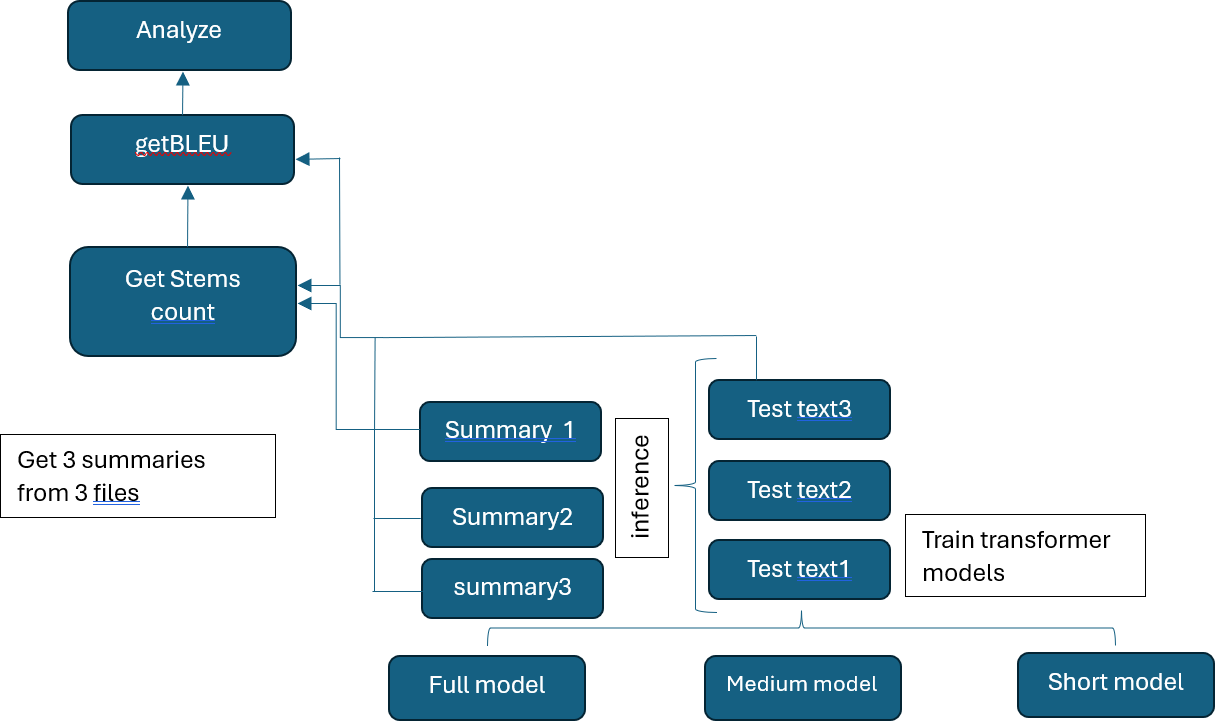
\includegraphics[width=0.8\textwidth]{assets/55}
	\caption*{Figure 1- Algorithm of representativeness analyze}
\end{figure}

\begin{multicols}{2}
Let\textquotesingle s look at the algorithm step by step:

1) The dataset was divided into parts, resulting in three datasets of
different sizes. Using these datasets, three transformer models were
trained {[}19{]}, with identical architecture, which differ only in the
training dataset. Let\textquotesingle s call them Full model, Medium
model, Short model respectively.

2) Test files of one training distribution were submitted to the input
of each model.

3) Word stems of training datasets and generated text files with
summaries were obtained using the application {[}20{]}. Standard
preprocessing is performed first - punctuation marks, words that are too
short, and abbreviations are removed.

4) Having received the numerical values, we will analyze the quality of
work and representativeness. The analysis consists of determining how
the number of word stems affects the performance and the
representativeness of the model. Representativeness in the case under
consideration - is as a metric of how the degree of representation of
the diversity of words is represented (full range of linguistics
distributions) affects operation of the summarization model. That is how
much does the BLEU estimate change when the number of stems changes
significantly.

5) The training corpus must contain a minimum of stems in order to be
considered representative. To do this, we determine the minimum at which
the text is readable and does not have repetition of words. \hl{}

Table 1 shows data on training datasets. Under the number of stems means
the number of unique stems. This data shows how our datasets in size.

\begin{table}[H]
\caption*{Table 1 - Train datasets statistics}
\centering
\begin{tabular}{|l|l|l|}
\hline
train dataset & stems & strings \\ \hline
Full model & 80137 & 240000 \\ \hline
Medium model & 26347 & 104772 \\ \hline
Short model & 18580 & 50000 \\ \hline
\end{tabular}
\end{table}

\emph{Training a neural network.} For training we use a transformer
model, trained with standard parameters for 12 epochs. Training dataset
- Simple English Wikipedia {[}21{]} which was translated into Kazakh
language. The training was carried out using the Google Colab system. We
trained separate neural networks on each obtained dataset and then
analyzed the quality on various news text files that did not contain
rare, specialized terms. Next, the so-called model inference was
performed - this is the process of creating summarization of a sentence
in the Kazakh language. The number words and unique word stems of the
source part of the files that were used for inference are given in the
table. 2.

\begin{table}[H]
\caption*{Table2 - Summary statistics for test files}
\centering
\begin{tabular}{|l|l|}
\hline
test file & stems \\ \hline
test text 1 & 168 \\ \hline
test text 2 & 386 \\ \hline
test text 3 & 86 \\ \hline
\end{tabular}
\end{table}
This data is necessary in order to assess how much the text has been
reduced and how representative the text is after summarization. Let us
consider the ratios of scores and the number of word stems obtained by
summarization in table 3.

\emph{Analysis of representativeness.} Table 3 contains columns of stems
and scores for each model. The columns of word stems show the degree of
file reduction taking into account representativeness. The first file
test text 1: Full model has a BLEU score of 60.39, Medium model has a
score of 35, Short model has a BLEU score of 28.88. Lowest number of
stems in a Short model - 78 stems, that is, a reduction of 54 percent
and at the same time the BLEU score decreased by 2 times.

Next the second file: Full model - 62.60, Medium model - 55, Short model
- 37.45. Lowest value of stems - Short model reduction by 33 percent.

The third file: Full model - 55. Medium model - 55 and Short model -
25.82. Word stems - Short model by 40 percent.

As we can see, in the case of the Short model, the text is shorter, but
the drop in score is very large. Scores are reduced by almost 50 percent
compared to the Full model. The Short model has scores at the level of
the Medium model, although it was trained on a dataset that was half as
large. There is no point in reducing the size of the training dataset
below. That is, the Short model, which contains less word stems, gives
almost the same results as the Medium model. The best results are on the
second file which contains the largest amount of stems and it has the
best BLEU scores in all three tests. There is a strong drop in ratings
on file 3, which is the smallest in size.
\end{multicols}


\begin{table}[H]
\caption*{Table 3 - BLEU scores and sample sizes by model}
\centering
\begin{tabular}{|l|ll|ll|ll|}
\hline
\multirow{2}{*}{test source file} & \multicolumn{2}{l|}{Medium model} & \multicolumn{2}{l|}{Full model stems} & \multicolumn{2}{l|}{Short model} \\ \cline{2-7}
 & \multicolumn{1}{l|}{Stems} & BLUE & \multicolumn{1}{l|}{stems} & BLUE & \multicolumn{1}{l|}{stems} & BLUE \\ \hline
test text 1 & \multicolumn{1}{l|}{106} & 35.72 & \multicolumn{1}{l|}{119} & 60.39 & \multicolumn{1}{l|}{78} & 28.88 \\ \hline
test text 2 & \multicolumn{1}{l|}{284} & 55.74 & \multicolumn{1}{l|}{306} & 62.60 & \multicolumn{1}{l|}{257} & 37.45 \\ \hline
test text 3 & \multicolumn{1}{l|}{78} & 54 & \multicolumn{1}{l|}{72} & 58 & \multicolumn{1}{l|}{51} & 25.82 \\ \hline
\end{tabular}
\end{table}

On all test files, the difference in the number of stems differs
slightly and all three files are reduced by approximately the same
number of stems. But at the same time, the decrease in scores is not
proportional to the decrease of stems and dataset size. On the third
file, the Full model shows a BLEU score of 58, and the Short model - 51.
The score has decreased, but on the Medium and Short models it is
approximately the same in all three cases, and the Short model reduces
the text more strongly in all examples.

Thus, the representative dataset shows good scores even with a
relatively small number of lines. Usually the volume of dictionaries is
sufficient for a good translation, for example, Miller's dictionary
contains 60 thousand words (the number of stems should be less). In our
case, the stem size is from 50,000 to 90,000. So, the training corpus
must contain more than 50,000 stems for it to be representative and for
the dataset to work.

Short model has a minimum size sufficient for correct summarization. In
the resulting text files, the model replaced some words and discarded
unimportant parts. Also, a common problem - repetition of words - is not
observed in the work of the models. Table 4 provides examples of
sentence reductions by each model. As we see in the case of the Short
model, we have the shortest summarization in the first and second
sentence.

\begin{figure}[H]
	\centering
	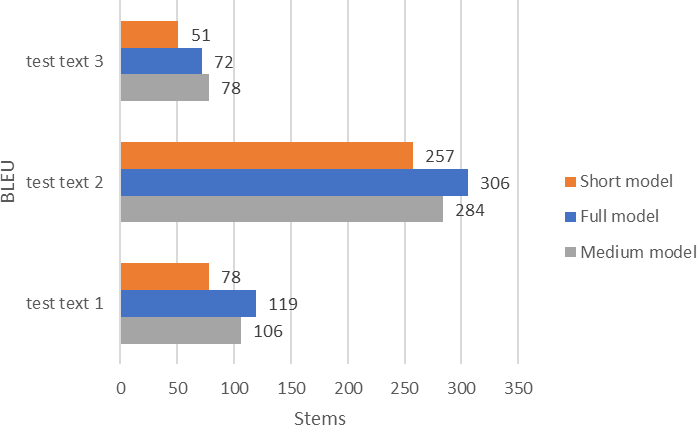
\includegraphics[width=0.6\textwidth]{assets/56}
	\caption*{Figure 2 - Resulting scores with the number of stems in test files}
\end{figure}

\begin{table}[H]
\caption*{Table 4 - Example of the received text on test file}
\centering
\begin{tabular}{|p{0.2\textwidth}|p{0.2\textwidth}|p{0.2\textwidth}|p{0.2\textwidth}|}
\hline
Оriginal sentence & Medium model & Short model & Full model \\ \hline
Шетелде демалу бізге керемет жаңа көңіл күй сыйлайды әрі күнделікті күйбең тіршіліктен біршама демалуға мүмкіндік береді. & Шетелде демалу бізге керемет жаңа көңіл күй әрі күнделікті күйбең тіршіліктен біршама демалуға мүмкіндік береді. & Ол демалу біршама біршама мүмкіндік мүмкіндік береді. & Фитнес-турлар - дене жаттығулары мен дүниежүзін саяхаттауды біріктіретін турлардың жалпы атауы. \\ \hline
Егер сіз спортты сүйсеңіз, саяхаттау кезінде әрі пайдалы іспен айналысып, әрі саяхаттап ерекше демалатын боласыз. & Егер сіз спортты сүйсеңіз, саяхаттау кезінде әрі пайдалы іспен айналысып, әрі саяхаттап ерекше демалатын & Егер сіз спортты сүйсеңіз, ашылуы кезінде басталады. & Егер сіз спортты сүйсеңіз, саяхаттау кезінде әрі пайдалы іспен айналысып, әрі келді, ерекше демалатын боласыз. \\ \hline
Фитнес-турлар – дене жаттығулары мен дүниежүзін саяхаттауды біріктіретін турлардың жалпы атауы. & Фитнес-турлар - дене жаттығулары мен дүниежүзін & Фитнес-турлар - дене шынықтыру мен дүниежүзін біріктіретін турлардың жалпы атауы. & Фитнес-турлар - дене жаттығулары мен дүниежүзін саяхаттауды біріктіретін турлардың жалпы атауы. \\ \hline
\end{tabular}
\end{table}

\begin{multicols}{2}
{\bfseries Conclusion}. In this work, the initial research hypothesis was:
is it possible to determine the representativeness of the training
dataset before conducting resource-intensive experiments on training a
neural model of the summarization problem? To solve this problem, the
number of stems in the dataset was used. Based on the experiments
performed, positive results were obtained confirming the original
hypothesis. During the work, three transformer models were obtained,
trained on datasets of different sizes. Taking the number of word stems
as a metric for the representativeness of a dataset, we analyzed the
dependence of the BLEU score on the different representativeness of the
dataset. Experimentally, graphs were obtained showing the influence of
the number of word stems on the operation of the summarization model.

From the results of the experiment, the conclusion was drawn that in
practical application it is necessary to pay attention to the diversity
of word stems; the more word stems, the better the model will work. To
determine the minimum suitable dataset size, the minimum size of the
training dataset was determined at which there is no significant drop in
the BLEU score on the dataset.

The practical application of the results of the work is relevant in the
field of creating and improving parallel corpora for training neural
models for languages \hspace{0pt}\hspace{0pt}with a small number of
resources, i.e. for low-resource languages. Since the summarization
problem belongs to the class of Sequence-to-Sequence problems, the
conclusion of this work can be extended to other problems of this class:
machine translation and other natural language processing tasks.
\end{multicols}

\begin{center}
{\bfseries References}
\end{center}

\begin{noparindent}
1.Leech G., Aijmer K., Altenberg B. The state of the art in corpus
linguistics. English corpus linguistics: studies in honour of Jan
Svartvik. London:Longman.-1991. -P.8-29

2. Tukeyev U., Karibayeva A.Inferring the Complete Set of Kazakh Endings
as a Language Resource. In: Hernes M., Wojtkiewicz K., Szczerbicki E.
(eds) Advances in Computational Collective Intelligence. ICCCI 2020.
Communications in Computer and Information Science.-2020.- Vol 1287.-
P.741-751. https://doi.org/10.1007/978-3-030-63119-2\_60

3.Papineni K.,~Roukos~S.,~Ward,T.~and~Zhu~W.J.~(2002). BLEU: A method
for automatic evaluation of machine translation. //Proceedings of
ACL-2002: 40th Annual meeting of the Association for Computational
Linguistics.-Philadelphia,Pennsylvania.-USA.-P.311--318. {[}Google
Scholar{]}

4.West.J, Ventura D.,Warnick S. Spring Research Presentation: a
Theoretical Foundation for Inductive Transfer. //Journal of Software
Engineering and Applications.-2007.- Vol.12 (11)

5.Pan Y.,Li X.,Yang Y., Dong R. Multi-Task Neural Model for
Agglutinative Language Translation. Proceedings of the 58th Annual
Meeting of the Association for Computational Linguistics:Student
Research Workshop.- 2020.- P.103-110 DOI 10.18653/v1/2020.acl-srw.15

6.Maimaiti M., Liu Y., Luan H., Sun M. ,Enriching the Transfer Learning
with Pre-Trained Lexicon Embedding for Low-Resource Neural Machine
Translation.//Tsinghua Sciences and Technology.-2022.-Vol.27.(1).-
P.150-163. DOI 10.26599/TST.2020.9010029

7.Kermanshahi M.A.,Akbari A.,Nasersharif B.Transfer Learning for
End-to-End ASR to Deal with Low-Resource Problem in Persian Language.//
2021 26th International Computer Conference, Computer Society of Iran
(CSICC). DOI:10.1109/CSICC52343.2021.9420540

8.Batuhan B., Tunga G. Turkish abstractive summarization using
pretrained sequence-to-sequence models. //Natural Language
Engineering.-2023.-Vol.29(5).- P.1275-1304

DOI 10.1017/S1351324922000195

9.Liu W., Xiao L., Jiang S., Li W. Language Resource Extension for
Indonesian-Chinese Machine Translation. //Conference:International
Conference on Asian Language Processing (IALP).-2018.

DOI:10.1109/IALP.2018.8629155

10.Jiang S., Fu S., Lin N., Fu Y.Pretrained Models and Evaluation Data
for the Khmer Language //Tsinghua Science and
Technology.-2022.-Vol.27(4).-P.-709-718.

DOI:10.26599/TST.2021.9010060

11.Maruyama T., Yamamoto K. Extremely Low Resource Text Simplification
with Pre-Trained Transformer Language Model // International Journal of
Asian Language Processing.-2020.-Vol.30(01):205001 DOI

10.1142/S2717554520500010

12.Parida S., Motlicek P. Abstract Text Summarization: A Low Resource
Challenge.// Proceedings of the 2019 Conference on Empirical Methods in
Natural Language Processing and the 9th International Joint Conference
on Natural Language Processing (EMNLP-IJCNLP).-2019.-P.5994-5998. DOI
10.18653/v1/D19-1616

13.Deshpande P., Jahirabadkar S. Study of Low Resource Language Document
Extractive Summarization using Lexical chain and Bidirectional Encoder
Representations from Transformers (BERT).// International Conference on
Computational Performance Evaluation (ComPE).-2021

DOI:10.1109/ComPE53109.2021.9751919

14.Paddington C., Cleghorn C.W. Improving transformer model translation
for low resource South African languages using BERT. 2021 IEEE Symposium
Series on Computational Intelligence (SSCI). DOI

10.1109/SSCI50451.2021.9659923

15.Alami N., Meknassi M., Ouatik S.A., Ennahnahi N.Impact of stemming on
Arabic text summarization.// 2016 4th IEEE International Colloquium on
Information Science and Technology (CiSt). DOI 10.1109/CIST.2016.7805067

16.Shams R., Elsayed A., Akter Q. M.-Z. A corpus-based evaluation of a
domainspecific text to knowledge mapping prototype.//Journal of
Computers.-2010.-Vol5(1).-P.69--80.

https://doi.org/10.4304/jcp.5.1.69-80

17.Zevallos R., Bel N. Hints on the data for language modeling of
synthetic languages with transformers. //Proceedings of the 61st Annual
Meeting of the Association for Computational Linguistics .-2023.-Vol.1:
Long Papers).-P.12508-12522.

DOI:10.18653/v1/2023.acl-long.699

18.U.A. Tukeyev, Vychislitelnaya morfologiya tyurkskikh yazykov.//
Uchebnoe posobie,Almaty: Kazak universiteti.- 2021.- pp. 11-13.{[}In
Russ.{]}

19.Vaswani A., Shazeer N., Parmar N., Uszkoreit J. Attention is all you
need.// \emph{Advances in neural information processing
systems.-2017.-P.5998-6008.} http://arxiv.org/abs/1706.03762

20.Stemming algorithm with stems lexicon according to the CSE morphology
model {[}Electronic resource{]}. Access mode:
https://github.com/nlp-KazNU

/Stemming\_algorithm\_with\_stems-lexicon\_according\_to\_the\_CSE\_morphology\_model.
Revised date:08.04.2024.

\phantomsection\label{kix.87gpl39zxgv2}{}21.Hwang W., Hajishirzi H.
Aligning sentences from standard wikipedia to simple wikipedia.
//Conference of the North American Chapter of the Association for
Computational Linguistics:Human Language Technologies. -2015.- P.
211-217. DOI:10.3115/v1/N15-1022
\end{noparindent}

\emph{{\bfseries Information about the authors}}

\begin{noparindent}
Zhabaev T.R.- мaster, Al-Farabi KazNU, Almaty, Kazakhstan, e-mail:
ltalgat14430@gmail.com;

Tukeyev U.A.- Doctor of Technical Sciences, Professor, Al-Farabi KazNU,
Almaty, Kazakhstan e-mail:

ualsher.tukeyev@gmail.com
\end{noparindent}

\emph{{\bfseries Сведения об авторах}}

\begin{noparindent}
Жабаев Т.Р.- магистр, кафедра ``Информационные системы'', КазНУ имени
аль-Фараби,e-mail:

talgat14430@gmail.com;

Тукеев У.А.- доктор технических наук, профессор, КазНУ имени аль-Фараби,
e-mail:

ualsher.tukeyev@gmail.com
\end{noparindent}
